\chapter{Quadratic functions}
\section{Defined on $\mdr$}
Let $f:\mdr \rightarrow \mdr, f(x) = a \cdot x^2 + b \cdot x + c$ with $a \in \mdr \setminus \Set{0}$ and 
$b, c \in \mdr$ be a quadratic function.

\begin{figure}[htp]
    \centering
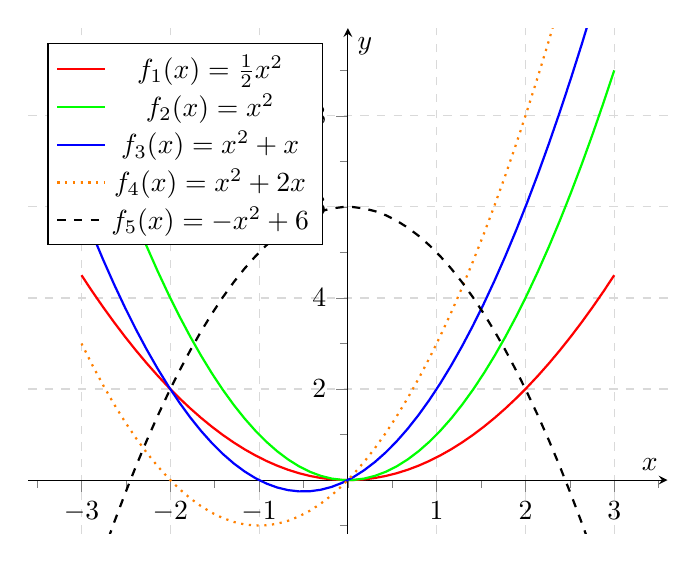
\begin{tikzpicture}
    \begin{axis}[
        legend pos=north west,
        axis x line=middle,
        axis y line=middle,
        grid = major,
        width=0.8\linewidth,
        height=8cm,
        grid style={dashed, gray!30},
        xmin=-3,    % start the diagram at this x-coordinate
        xmax= 3,    % end   the diagram at this x-coordinate
        ymin=-0.25, % start the diagram at this y-coordinate
        ymax= 9,    % end   the diagram at this y-coordinate
        axis background/.style={fill=white},
        xlabel=$x$,
        ylabel=$y$,
        tick align=outside,
        minor tick num=-3,
        enlargelimits=true,
        tension=0.08]
      \addplot[domain=-3:3, thick,samples=50, red]    {0.5*x*x}; 
      \addplot[domain=-3:3, thick,samples=50, green]  { x*x}; 
      \addplot[domain=-3:3, thick,samples=50, blue]   { x*x +   x};
      \addplot[domain=-3:3, thick,samples=50, orange,dotted] { x*x + 2*x};
      \addplot[domain=-3:3, thick,samples=50, black,dashed]  {-x*x + 6};
      \addlegendentry{$f_1(x)=\frac{1}{2}x^2$}
      \addlegendentry{$f_2(x)=x^2$}
      \addlegendentry{$f_3(x)=x^2+x$}
      \addlegendentry{$f_4(x)=x^2+2x$}
      \addlegendentry{$f_5(x)=-x^2+6$}
    \end{axis} 
\end{tikzpicture}
    \caption{Quadratic functions}
\end{figure}

\subsection{Calculate points with minimal distance}
In this case, $d_{P,f}^2$ is polynomial of degree $n^2 = 4$. 
We use Theorem~\ref{thm:fermats-theorem}:\nobreak
\begin{align}
    0     &\overset{!}{=} (d_{P,f}^2)'\\
          &= 2x -2 x_p -2y_p f'(x) + \left (f(x)^2 \right )'\\
          &= 2x -2 x_p -2y_p f'(x) + 2 f(x) \cdot f'(x) \rlap{\hspace*{3em}(chain rule)}\label{eq:minimizingFirstDerivative}\\
\Leftrightarrow 0 &\overset{!}{=} x -x_p -y_p f'(x) + f(x) \cdot f'(x) \rlap{\hspace*{3em}(divide by 2)}\label{eq:minimizingFirstDerivative}\\
          &= x -x_p -y_p (2ax+b) + (ax^2+bx+c)(2ax+b)\\
          &= x -x_p -y_p \cdot 2ax- y_p b + (2 a^2 x^3+2 a b x^2+2 a c x+ab x^2+b^2 x+bc)\\
          &= x -x_p -2y_p ax- y_p b + (2a^2 x^3 + 3 ab x^2 + 2acx + b^2 x + bc)\\
          &= 2a^2 x^3 + 3 ab x^2 + (1 -2y_p a+ 2ac + b^2)x +(bc-by_p-x_p)\label{eq:quadratic-derivative-eq-0}
\end{align}

This is an algebraic equation of degree 3.
There can be up to 3 solutions in such an equation. Those solutions
can be found with a closed formula. But not every solution of the
equation given by Theorem~\ref{thm:fermats-theorem}
has to be a solution to the given problem as you can see in
Example~\ref{ex:false-positive}.
\goodbreak
\begin{example}\label{ex:false-positive}
    Let $a = 1,  b = 0,  c=-1, x_p= 0, y_p = 1$.
    So $f(x) = x^2 - 1$ and $P(0, 1)$.
    \begin{align}
        \xRightarrow{\text{Equation}~\ref{eq:quadratic-derivative-eq-0}} 0 &\stackrel{!}{=} 2x^3 - 3x\\
        &= x(2x^2-3)\\
        \Rightarrow x_{1,2} &= \pm \sqrt{\frac{3}{2}} \text{ and } x_3 = 0\\
        d_{P,f}(x_3) &= \sqrt{0^2 + (-1-1)^2} = 2\\
        d_{P,f} \left (\pm \sqrt{\frac{3}{2}} \right ) &= \sqrt{\left (\sqrt{\frac{3}{2} - 0} \right )^2 + \left (\frac{1}{2}-1 \right )^2}\\
            &= \sqrt{\nicefrac{3}{2}+\nicefrac{1}{4}} \\
            &= \sqrt{\nicefrac{7}{4}}\\
    \end{align}
    This means $x_3$ is not a point of minimal distance, although
    $(d_{P,f}(x_3))' = 0$.
\end{example}


\subsection{Number of points with minimal distance}
\begin{theorem}
    A point $P$ has either one or two points on the graph of a 
    quadratic function $f$ that are closest to $P$.
\end{theorem}

\begin{proof}
The number of closests points of $f$ cannot be bigger than 3, because
Equation~\ref{eq:quadratic-derivative-eq-0} is a polynomial function
of degree 3. Such a function can have at most 3 roots. As $f$ has
at least one point on its graph, there is at least one point with
minimal distance.

In the following, I will do some transformations with $f = f_0$ and
$P = P_0$. This will make it easier to calculate the minimal distance
points. Moving $f_0$ and $P_0$ simultaneously in $x$ or $y$ direction does 
not change the minimum distance. Furthermore, we can find the 
points with minimum distance on the moved situation and calculate
the minimum points in the original situation.

First of all, we move $f_0$ and $P_0$ by $\frac{b}{2a}$ in $x$ direction, so
\[f_1(x) = ax^2 - \frac{b^2}{4a} + c \;\;\;\text{ and }\;\;\; P_1 = \left (x_p+\frac{b}{2a},\;\; y_p \right )\]

Because:\footnote{The idea why you subtract $\frac{b}{2a}$ within
$f$ is that when you subtract something from $x$ before applying
$f$ it takes more time ($x$ needs to be bigger) to get to the same
situation. In consequence, if we want to move the whole graph by 1 
to the left, we have to add $+1$.}
\begin{align}
    f(x-\nicefrac{b}{2a}) &= a (x-\nicefrac{b}{2a})^2 + b (x-\nicefrac{b}{2a}) + c\\
    &= a (x^2 - \nicefrac{b}{a} x + \nicefrac{b^2}{4a^2}) + bx - \nicefrac{b^2}{2a} + c\\
    &= ax^2 - bx + \nicefrac{b^2}{4a} + bx - \nicefrac{b^2}{2a} + c\\
    &= ax^2 -\nicefrac{b^2}{4a} + c
\end{align}


Then move $f_1$ and $P_1$ by $\frac{b^2}{4a}-c$ in $y$ direction. You get:
\[f_2(x) = ax^2\;\;\;\text{ and }\;\;\; P_2 = \Big (\underbrace{x_P+\frac{b}{2a}}_{=: z},\;\; \underbrace{y_P+\frac{b^2}{4a}-c}_{=: w} \Big )\]

As $f_2(x) = ax^2$ is symmetric to the $y$ axis, only points 
$P = (0, w)$ could possilby have three minima.

Then compute:
\begin{align}
  d_{P,{f_2}}(x)  &= \sqrt{(x-0)^2 + (f_2(x)-w)^2}\\
    &= \sqrt{x^2 + (ax^2-w)^2}\\
    &= \sqrt{x^2 + a^2 x^4-2aw x^2+w^2}\\
    &= \sqrt{a^2 x^4 + (1-2aw) x^2 + w^2}\\
    &= \sqrt{\left (a x^2 + \frac{1-2 a w}{2a} \right )^2 + w^2 - \left (\frac{1-2 a w}{2a} \right )^2}\\
    &= \sqrt{\left (a x^2 + \nicefrac{1}{2a}- w \right )^2 + \left (w^2 - \left (\frac{1-2 a w}{2a} \right )^2 \right)}
\end{align}

This means, the term
\[a^2 x^2 + (\nicefrac{1}{2a}- w)\]
has to get as close to $0$ as possilbe when we want to minimize 
$d_{P,{f_2}}$. For $w \leq \nicefrac{1}{2a}$ you only have $x = 0$ as a minimum.
For all other points $P = (0, w)$, there are exactly two minima $x_{1,2} = \pm \sqrt{\frac{\frac{1}{2a} - w}{a}}$.
$\qed$
\end{proof}

\subsection{Solution formula}
We start with the graph that was moved so that $f_2 = ax^2$.

\textbf{Case 1:} $P$ is on the symmetry axis, hence $x_P = - \frac{b}{2a}$.

In this case, we have already found the solution. If $w = y_P + \frac{b^2}{4a} - c > \frac{1}{2a}$,
then there are two solutions:
\[x_{1,2} = \pm \sqrt{\frac{\frac{1}{2a} - w}{a}}\]
Otherwise, there is only one solution $x_1 = 0$.

\textbf{Case 2:} $P = (z, w)$ is not on the symmetry axis, so $z \neq 0$. Then you compute:
\begin{align}
  d_{P,{f_2}}(x)  &= \sqrt{(x-z)^2 + (f(x)-w)^2}\\
    &= \sqrt{(x^2 - 2zx + z^2) + ((ax^2)^2 - 2 awx^2 + w^2)}\\
    &= \sqrt{a^2x^4 + (1- 2 aw)x^2 +(- 2z)x + z^2 + w^2}\\
  0 &\stackrel{!}{=} \Big(\big(d_{P, {f_2}}(x)\big)^2\Big)' \\
    &= 4a^2x^3 + 2(1- 2 aw)x +(- 2z)\\
    &= 2 \left (2a^2x^3 + (1- 2 aw)x \right ) - 2z\\
    \Leftrightarrow 0 &\stackrel{!}{=} 2a^2x^3  + (1- 2 aw) x - z\\
\stackrel{a \neq 0}{\Leftrightarrow} 0 &\stackrel{!}{=} x^3 + \underbrace{\frac{1- 2 aw}{2 a^2}}_{=: \alpha} x  + \underbrace{\frac{-z}{2 a^2}}_{=: \beta}\\
    &= x^3 + \alpha x + \beta\label{eq:simple-cubic-equation-for-quadratic-distance}
\end{align}

Let $t$ be defined as
\[t := \sqrt[3]{\sqrt{3 \cdot (4 \alpha^3 + 27 \beta^2)} -9\beta}\]

\subsubsection{Analyzing $t$}
\begin{align}
    t &:= \sqrt[3]{\sqrt{3 \cdot (4 \alpha^3 + 27 \beta^2)} -9\beta}\\
    &= \sqrt[3]{\sqrt{3 \cdot \left (4 \left (\frac{1- 2 aw}{2 a^2} \right )^3 + 27 \left (\frac{-z}{2 a^2} \right )^2 \right )} -9 \frac{-z}{2 a^2}}\\
    &= \sqrt[3]{\sqrt{3 \cdot \left (4 \left (\frac{1- 2 a (y_P+\frac{b^2}{4a}-c)}{2 a^2} \right )^3 + 27 \left (\frac{-(x_P+\frac{b}{2a})}{2 a^2} \right )^2 \right )} 
    -9 \frac{-(x_P+\frac{b}{2a})}{2 a^2}}\\
    &= \sqrt[3]{\sqrt{12a^4 \cdot \left (4 \frac{\left ( 1- 2 a (y_P+\frac{b^2}{4a}-c) \right )^3}{2 a^2}  + 27 \left (x_P^2+2 x_P \frac{b}{2a} + \frac{b^2}{4a^2} \right )\right )}
    + 9 \frac{x_P+\frac{b}{2a}}{2 a^2}}\\
    &= \sqrt[3]{\sqrt{\frac{12a^4}{4a^2} \left (8 \left ( 1- 2 a (y_P+\frac{b^2}{4a}-c) \right )^3  + 27 (4 a^2 x_P^2+4a x_P \frac{b}{2a} + b^2 )\right )}
    + 9 \frac{x_P+\frac{b}{2a}}{2 a^2}}\\
    &= \sqrt[3]{\sqrt{3a^2 \left (8 \left ( 1- 2 a (y_P+\frac{b^2}{4a}-c) \right )^3  + 27 (4 a^2 x_P^2+4a x_P \frac{b}{2a} + b^2 )\right )}
    + 9 \frac{x_P+\frac{b}{2a}}{2 a^2}}
\end{align}

\todo[inline]{When is $t = 0$? When is $t \in \mdr$?}


\subsubsection{Solutions of $x^3 + \alpha x + \beta$}
I will make use of the following identities:
\begin{align*}
    (1-i \sqrt{3})^2     &= -2 (1+i \sqrt{3})\\
    (1+i \sqrt{3})^2     &= -2 (1-i \sqrt{3})\\
    (1 \pm i \sqrt{3})^3 &= -8\\
    (a-b)^3              &= a^3-3 a^2 b+3 a b^2-b^3
\end{align*}

\textbf{Case 2.1:} 
$4 \alpha^3 + 27 \beta^2 \geq 0$:
One solution of Equation~\ref{eq:simple-cubic-equation-for-quadratic-distance}
is
\[x = \frac{t}{\sqrt[3]{18}} - \frac{\sqrt[3]{\frac{2}{3}} \alpha }{t}\]

When you insert this in Equation~\ref{eq:simple-cubic-equation-for-quadratic-distance}
you get:\footnote{Remember: $(a-b)^3 = a^3-3 a^2 b+3 a b^2-b^3$}
\allowdisplaybreaks
\begin{align}
    0 &\stackrel{!}{=} \left (\frac{t}{\sqrt[3]{18}} - \frac{\sqrt[3]{\frac{2}{3}} \alpha }{t} \right )^3 + \alpha \left (\frac{t}{\sqrt[3]{18}} - \frac{\sqrt[3]{\frac{2}{3}} \alpha }{t} \right ) + \beta\\
&= (\frac{t}{\sqrt[3]{18}})^3 
    - 3 (\frac{t}{\sqrt[3]{18}})^2 \frac{\sqrt[3]{\frac{2}{3}} \alpha }{t} 
    + 3 (\frac{t}{\sqrt[3]{18}})(\frac{\sqrt[3]{\frac{2}{3}} \alpha }{t})^2 
    - (\frac{\sqrt[3]{\frac{2}{3}} \alpha }{t})^3 
    + \alpha \left (\frac{t}{\sqrt[3]{18}} - \frac{\sqrt[3]{\frac{2}{3}} \alpha }{t} \right ) + \beta\\
&= \frac{t^3}{18}             
    - \frac{3t^2}{\sqrt[3]{18^2}} \frac{\sqrt[3]{\frac{2}{3}} \alpha }{t}
    + \frac{3t}{\sqrt[3]{18}} \frac{\sqrt[3]{\frac{4}{9}} \alpha^2 }{t^2} 
    - \frac{\frac{2}{3} \alpha^3 }{t^3} 
    + \alpha \left (\frac{t}{\sqrt[3]{18}} - \frac{\sqrt[3]{\frac{2}{3}} \alpha }{t} \right ) + \beta\\
&= \frac{t^3}{18}
    - \frac{\sqrt[3]{18} t \alpha}{\sqrt[3]{18^2}}
    + \frac{\sqrt[3]{12} \alpha^2}{\sqrt[3]{18} t}  
    - \frac{2 \alpha^3 }{3t^3} 
    + \alpha \left (\frac{t}{\sqrt[3]{18}} - \frac{\sqrt[3]{\frac{2}{3}} \alpha }{t} \right ) + \beta\\
&= \frac{t^3}{18} 
    - \frac{t \alpha}{\sqrt[3]{18}} 
    \color{red}+ \frac{\sqrt[3]{2} \alpha^2}{\sqrt[3]{3} t} \color{black}
    - \frac{2 \alpha^3 }{3 t^3} 
    + \color{red}\alpha \color{black} \left (\frac{t}{\sqrt[3]{18}}  \color{red}- \frac{\sqrt[3]{\frac{2}{3}} \alpha }{t} \color{black}\right ) 
    + \beta\\
&= \frac{t^3}{18} \color{blue}- \frac{t \alpha}{\sqrt[3]{18}} \color{black} 
    - \frac{2 \alpha^3 }{3 t^3} 
    \color{blue}+ \frac{\alpha t}{\sqrt[3]{18}} \color{black} 
    + \beta\\
&= \frac{t^3}{18} - \frac{2 \alpha^3 }{3 t^3} + \beta\\
&= \frac{t^6 - 12 \alpha^3 + \beta 18 t^3}{18t^3}
\end{align}

Now only go on calculating with the numerator. Start with resubstituting
$t$:
\begin{align}
0 &= (\sqrt{3 \cdot (4 \alpha^3 + 27 \beta^2)} -9\beta)^2 - 12 \alpha^3 + \beta 18 (\sqrt{3 \cdot (4 \alpha^3 + 27 \beta^2)} -9\beta)\\
&= (\sqrt{3 \cdot (4 \alpha^3 + 27 \beta^2)})^2 +(9\beta)^2 - 12 \alpha^3 -(2 \cdot 9)\cdot 9\beta^2\\
&= 3 \cdot (4 \alpha^3 + 27 \beta^2) -81 \beta^2 - 12 \alpha^3\\
&= 0
\end{align}

\goodbreak
\textbf{Case 2.2:}
The second solution of $x^3+\alpha x + \beta=0$ is
\[x = \frac{(1+i \sqrt{3})\alpha}{\sqrt[3]{12} \cdot t}
     -\frac{(1-i\sqrt{3}) t}{2\sqrt[3]{18}}\]

We will verify it in multiple steps. First, calculate $x^3$:
\begin{align}
    x^3 &= \underbrace{\left (\frac{(1+i\sqrt{3})\alpha}{\sqrt[3]{12} \cdot t} \right)^3}_{=: \raisebox{.5pt}{\textcircled{\raisebox{-.9pt} {1}}}}
           \underbrace{- 3 \left(\frac{(1+i\sqrt{3})\alpha}{\sqrt[3]{12} \cdot t} \right)^2 \left(\frac{(1-i\sqrt{3})t}{2 \sqrt[3]{18}} \right)}_{=: \raisebox{.5pt}{\textcircled{\raisebox{-.9pt} {2}}}}\\
         &\hphantom{{}=}+ \underbrace{3 \left(\frac{(1+i\sqrt{3})\alpha}{\sqrt[3]{12} \cdot t} \right) \left(\frac{(1-i\sqrt{3})t}{2 \sqrt[3]{18}}\right)^2}_{=: \raisebox{.5pt}{\textcircled{\raisebox{-.9pt} {3}}}}
           \underbrace{- \left(\frac{(1-i\sqrt{3})t}{2 \sqrt[3]{18}}\right)^3}_{=: \raisebox{.5pt}{\textcircled{\raisebox{-.9pt} {4}}}}
\end{align}

Now simplify the summands of $x^3$:
\begin{align}
    \raisebox{.5pt}{\textcircled{\raisebox{-.9pt} {1}}} &=
    \left (\frac{(1+i\sqrt{3})\alpha}{\sqrt[3]{12} \cdot t} \right)^3\\
    &= \frac{-8\alpha^3}{12 t^3}\\
    &= \frac{-2 \alpha^3}{3 t^3}\\
    \raisebox{.5pt}{\textcircled{\raisebox{-.9pt} {2}}} &=- 3 \left(\frac{(1+i\sqrt{3})\alpha}{\sqrt[3]{12} \cdot t} \right)^2 \left(\frac{(1-i\sqrt{3})t}{2 \sqrt[3]{18}} \right)\\
    &= \frac{-3\alpha^2(-2(1-i\sqrt{3}))(1-i\sqrt{3})t}{t^2 \sqrt[3]{2^4 \cdot 3^2} \cdot 2 \sqrt[3]{2 \cdot 3^2}}\\
    &= \frac{6\alpha^2 t (-2 (1+i \sqrt{3}))}{12 t^2 \sqrt[3]{12}}\\
    &= \frac{- \alpha^2 (1+i\sqrt{3})}{t\sqrt[3]{12}}\\
    \raisebox{.5pt}{\textcircled{\raisebox{-.9pt} {3}}} &= 3 \left(\frac{(1+i\sqrt{3})\alpha}{\sqrt[3]{12} \cdot t} \right) \left(\frac{(1-i\sqrt{3})t}{2 \sqrt[3]{18}}\right)^2\\
    &= \frac{3\alpha t (1+i\sqrt{3})(-2(1+i\sqrt{3}))}{4 \cdot \sqrt[3]{12 \cdot 18^2}}\\
    &= \frac{-\alpha t (-2 (1 - i \sqrt{3}))}{2 \sqrt[3]{12 \cdot 4 \cdot 3}}\\
    &= \frac{\alpha t (1-i\sqrt{3})}{\sqrt[3]{2^4 \cdot 3^2}}\\
    &= \frac{\alpha t (1-i\sqrt{3}}{2 \sqrt[3]{18}}\\
    \raisebox{.5pt}{\textcircled{\raisebox{-.9pt} {4}}} &= - \left(\frac{(1-i\sqrt{3})t}{2 \sqrt[3]{18}}\right)^3\\
    &=- \frac{(-8) t^3}{8 \cdot 18}\\
    &= \frac{t^3}{18}
\end{align}

Now get back to the original equation:
\begin{align}
    0 &\stackrel{!}{=} x^3 + \alpha x + \beta \\
       &= \left (\frac{-2 \alpha^3}{3 t^3}
        + \color{red}\frac{-\alpha^2(1+\sqrt{3}i)}{t\sqrt[3]{12}}\color{black}
        + \color{blue}\frac{\alpha t(1-\sqrt{3}i)}{2\sqrt[3]{18}}\color{black}
        + \frac{t^3}{18} \right )\\
    &\hphantom{{}=} + \alpha \left (\color{red}\frac{(1+i \sqrt{3})\alpha}{\sqrt[3]{12} \cdot t} \color{black}
     \color{blue}-\frac{(1-i\sqrt{3}) t}{2\sqrt[3]{18}} \color{black} \right ) + \beta\\
    &= \frac{-2 \alpha^3}{3 t^3}
    + \frac{t^3}{18}
    + \beta\\
    &= \frac{-12 \alpha^3 + t^6+18 t^3 \beta}{18t^3}
\end{align}

Now continue with only the numerator
\begin{align}
    0 &\stackrel{!}{=}
    - 12 \alpha^3 
    + (\sqrt{3(4 \alpha^3 + 27 \beta^2)}-9\beta)^2
    + 18 (\sqrt{3(4 \alpha^3 + 27 \beta^2)} - 9 \beta) \beta\\
    &= 
    \color{red}- 12 \alpha^3 \color{black}+
    \left (
        3(\color{red}4 \alpha^3\color{black} + \color{blue}27 \beta^2 \color{black})
        \color{orange}- 2 \cdot \sqrt{3(4 \alpha^3 + 27 \beta^2)} \cdot 9\beta\color{black}
        + \color{blue}81 \beta^2\color{black}
    \right )\\
    &\hphantom{{}=}+ 18 \beta (\color{orange}\sqrt{3(4 \alpha^3 + 27 \beta^2)}\color{black} \color{blue}- 9 \beta\color{black}) \\
    &= 81 \beta^2 + 81 \beta^2 - 2 \cdot 81 \beta^2\\
    &= 0
\end{align}


\textbf{Case 2.3:}
One solution is
\[x = \frac{(1-i \sqrt{3}) \alpha}{\sqrt[3]{12} \cdot t}
     -\frac{(1+i\sqrt{3}) t}{2\sqrt[3]{18}}\]

We will verify it in multiple steps. First, get $x^3$:
\begin{align}
    x^3 &= \left (\frac{(1-i \sqrt{3}) \alpha}{\sqrt[3]{12} \cdot t} - \frac{(1+i\sqrt{3}) t}{2\sqrt[3]{18}} \right)^3\\
    &= \left (\frac{(2\sqrt[3]{18})(1-i \sqrt{3}) \alpha - (\sqrt[3]{12} \cdot t)(1+i\sqrt{3}) t}{\sqrt[3]{12} t \cdot 2 \sqrt[3]{18}} \right)^3\\
    &= \left (\frac{2\sqrt[3]{18}\alpha (1-i \sqrt{3}) - \sqrt[3]{12} t^2(1+i\sqrt{3})}{2t \cdot 6} \right )^3\\
    &= \bigg (\frac{\overbrace{\sqrt[3]{12} \alpha (1-i \sqrt{3}) - t^2 (1+i\sqrt{3})}^{\text{numerator}}}{\sqrt[3]{12^2} t} \bigg )^3
\end{align}

Now calculate numerator$^3$:
\begin{align}
    \left (\sqrt[3]{12} \alpha (1-i \sqrt{3}) - t^2(1+i\sqrt{3}) \right )^3 &= 
    12 \alpha^3 (1-i\sqrt{3})^3 \\
    &\hphantom{{}=}- 3 \sqrt[3]{12^2} \alpha^2(1-i\sqrt{3})^2 (t^2(1+i \sqrt{3}))\\
    &\hphantom{{}=}+ 3 \sqrt[3]{12\hphantom{^2}} \alpha\hphantom{^2} (1-i\sqrt{3}) t^4 (1+i\sqrt{3})^2 - t^6 (1+i\sqrt{3})^3\\
    &= 12 \alpha^3 \cdot (-8) \\
    &\hphantom{{}=}- 3 \sqrt[3]{12^2} \alpha^2(-2(1+i\sqrt{3}))(t^2(1+i \sqrt{3}))\\
    &\hphantom{{}=}+ 3 \sqrt[3]{12} \alpha (1-i\sqrt{3}) t^4 (-2(1-i\sqrt{3})) - t^6 (-8)\\
    &= -96 \alpha^3 + 6 \sqrt[3]{12^2} \alpha^2 t^2 (1+i \sqrt{3})^2\\
    &\hphantom{{}=}- 6 \sqrt[3]{12} \alpha t^4 (1-i\sqrt{3})^2 +8 t^6\\
    &= -96 \alpha^3 - 12 \sqrt[3]{12^2} \alpha^2 t^2 (1-i \sqrt{3})\\
    &\hphantom{{}=}+ 12 \sqrt[3]{12} \alpha t^4 (1+i \sqrt{3}) +8 t^6\\
    &= -96 \alpha^3 - 24 \sqrt[3]{18} \alpha^2 t^2 (1-i \sqrt{3})\\
    &\hphantom{{}=}+ 12 \sqrt[3]{12} \alpha t^4 (1+i \sqrt{3}) +8 t^6
\end{align}
\goodbreak
Now back to the original equation:
\begin{align}
0 &\stackrel{!}{=} x^3 + \alpha x + \beta\\
  &= \frac{-96 \alpha^3 - 24 \sqrt[3]{18} \alpha^2 t^2 (1-i \sqrt{3}) + 12 \sqrt[3]{12} \alpha t^4 (1+i \sqrt{3}) +8 t^6}{12^2 t^3}\\
  &\hphantom{{}=}+\alpha \left (\sqrt[3]{12} \cdot \frac{\sqrt[3]{12} \alpha (1-i \sqrt{3}) - t^2(1+i\sqrt{3})}{12t} \right ) + \beta
\end{align}

\todo[inline]{the calculation above seems to be wrong / too long. Next try}

When you insert this in Equation~\ref{eq:simple-cubic-equation-for-quadratic-distance}
you get:\footnote{Remember, that $(1+i\sqrt{3})^2 = -2 (1-i \sqrt{3})$ and $(1-i \sqrt{3})^2 = -2 (1+i \sqrt{3})$
and $(1 \pm i \sqrt{3})^3 = -8$}
\begin{align}
 0 &\stackrel{!}{=} \left( \frac{(1-i \sqrt{3}) \alpha}{\sqrt[3]{12} \cdot t}
     -\frac{(1+i\sqrt{3}) t}{2\sqrt[3]{18}} \right)^3 
     + \alpha \left ( \frac{(1-i \sqrt{3}) \alpha}{\sqrt[3]{12} \cdot t} -\frac{(1+i\sqrt{3}) t}{2\sqrt[3]{18}}\right )
     + \beta\\%%%%%%%%%%%%%%%%%%%%%%%%%%%%%
    &= \frac{(1-i \sqrt{3})^3 \alpha^3}{12 \cdot t^3}
       - 3 \left (\frac{(1-i \sqrt{3}) \alpha}{\sqrt[3]{12} \cdot t} \right )^2 \frac{(1+i\sqrt{3}) t}{2\sqrt[3]{18}}
       + 3 \frac{(1-i \sqrt{3}) \alpha}{\sqrt[3]{12} \cdot t} \left (\frac{(1+i\sqrt{3}) t}{2\sqrt[3]{18}} \right)^2\\
    &\hphantom{{}=}
       + \frac{(1+i\sqrt{3})^3 t^3}{2^3 \cdot 18}
       + \alpha \left ( \frac{(1-i \sqrt{3}) \alpha}{\sqrt[3]{12} \cdot t} -\frac{(1+i\sqrt{3}) t}{2\sqrt[3]{18}}\right )
       + \beta\\%%%%%%%%%%%%%%%%%%%%%%%%%%%%%
    &= \frac{-8 \alpha^3}{12t^3}
       - 3 \frac{-2(1+i \sqrt{3}) \alpha^2}{\sqrt[3]{12^2} t^2} \frac{(1+i\sqrt{3}) t}{2\sqrt[3]{18}}
       + 3 \frac{(1-i \sqrt{3}) \alpha}{\sqrt[3]{12} \cdot t} \frac{-2(1-i\sqrt{3}) t^2}{4\sqrt[3]{18^2}}\\
    &\hphantom{{}=}
       + \frac{-8 t^3}{2^3 \cdot 18}
       + \alpha \left ( \frac{(1-i \sqrt{3}) \alpha}{\sqrt[3]{12} \cdot t} -\frac{(1+i\sqrt{3}) t}{2\sqrt[3]{18}}\right )
       + \beta\\%%%%%%%%%%%%%%%%%%%%%%%%%%%%%
    &= \frac{-2 \alpha^3}{3t^3}
       + \frac{6 \alpha^2 t (-2)(1-i \sqrt{3})}{(\sqrt[3]{12^2} t^2)(2\sqrt[3]{18})}
       + \frac{12 \alpha t^2 (1+i \sqrt{3})}{(\sqrt[3]{12} \cdot t)(4\sqrt[3]{18^2)}}\\
    &\hphantom{{}=}
       + \frac{- t^3}{18}
       + \alpha \left ( \frac{(1-i \sqrt{3}) \alpha}{\sqrt[3]{12} \cdot t} -\frac{(1+i\sqrt{3}) t}{2\sqrt[3]{18}}\right )
       + \beta\\%%%%%%%%%%%%%%%%%%%%%%%%%%%%%
    &= \frac{-2 \alpha^3}{3t^3}
       + \frac{-6 \alpha^2 (1-i \sqrt{3})}{6 \sqrt[3]{12} t}
       + \frac{3 \alpha t (1+i \sqrt{3})}{6\sqrt[3]{18}}
       + \frac{- t^3}{18}\\
    &\hphantom{{}=}+ \alpha \left ( \frac{(1-i \sqrt{3}) \alpha}{\sqrt[3]{12} \cdot t} -\frac{(1+i\sqrt{3}) t}{2\sqrt[3]{18}}\right )
       + \beta\\%%%%%%%%%%%%%%%%%%%%%%%%%%%%%
    &= \frac{-2 \alpha^3}{3t^3}
       + \frac{-\alpha^2 (1-i \sqrt{3})}{\sqrt[3]{12} t}
       + \frac{\alpha t (1+i \sqrt{3})}{2\sqrt[3]{18}}
       + \frac{- t^3}{18}\\
    &\hphantom{{}=}+ \alpha \left ( \frac{(1-i \sqrt{3}) \alpha}{\sqrt[3]{12} \cdot t} -\frac{(1+i\sqrt{3}) t}{2\sqrt[3]{18}}\right )
       + \beta\\%%%%%%%%%%%%%%%%%%%%%%%%%%%%%
    &= \frac{12 \cdot (-2 \alpha^3) +(6 \sqrt[3]{18}t^2)(-\alpha^2 (1-i \sqrt{3}))+ (3 \sqrt[3]{12})(\alpha t (1+i \sqrt{3})) + (2t^3)(- t^3)}{36t^3}\\
    &\hphantom{{}=}+ \frac{(6 \sqrt[3]{18})((1-i \sqrt{3}) \alpha) - (3 \sqrt[3]{12})((1+i\sqrt{3}) t) + 36t^3 \beta}{36t^3}\\%%%%%%%%%%%%%%%%%%%%%%%%%%%%%
\end{align}

\goodbreak
Now calculate only the numerator:
\begin{align}
    0 &\stackrel{!}{=} -12 \alpha^3 - 6 \sqrt[3]{18} t^2 \alpha^2 (1 - i \sqrt{3})
        + 3 \sqrt[3]{12} \alpha t (1+i\sqrt{3}) - 2t^6\\
      &\hphantom{{}=} + 6\sqrt[3]{18} \alpha (1- i \sqrt{3})
        - 3 \sqrt[3]{12} t (1+i \sqrt{3}) + 36 t^3 \beta
\end{align}


\goodbreak
So the solution is given by
\todo[inline]{NO! Currently, there are erros in the solution.
Check $f(x) = x^2$ and $P=(-2,4)$. Solution should be $x_1 = -2$, but it isn't!}
\begin{align*}
x_S &:= - \frac{b}{2a} \;\;\;\;\; \text{(the symmetry axis)}\\
w &:= y_P+\frac{b^2}{4a}-c \;\;\; \text{ and } \;\;\; z := x_P+\frac{b}{2a}\\
\alpha &:= \frac{1- 2 aw}{2 a^2} \;\;\;\text{ and }\;\;\; \beta := \frac{-z}{2 a^2}\\
t &:= \sqrt[3]{\sqrt{3 \cdot (4 \alpha^3 + 27 \beta^2)} -9\beta}\\
\underset{x\in\mdr}{\arg \min d_{P,f}(x)} &= \begin{cases}
     x_1 = +\sqrt{a (y_p + \frac{b^2}{4a} - c) - \frac{1}{2}} + x_S \text{ and }   &\text{if } x_P = x_S \text{ and } y_p + \frac{b^2}{4a} - c >  \frac{1}{2a} \\
     x_2 = -\sqrt{a (y_p + \frac{b^2}{4a} - c) - \frac{1}{2}} + x_S\\
     x_1 = x_S   &\text{if } x_P = x_S \text{ and } y_p + \frac{b^2}{4a} - c \leq  \frac{1}{2a} \\
     x_1 = \frac{t}{\sqrt[3]{18}} - \frac{\sqrt[3]{\frac{2}{3}} \alpha }{t}   &\text{if } x_P \neq x_S
    \end{cases}
\end{align*}
\clearpage

\section{Defined on a closed interval $[a,b] \subseteq \mdr$}
Now the problem isn't as simple as with constant and linear
functions.

If one of the minima in $S_2(P,f)$ is in $[a,b]$, this will be the
shortest distance as there are no shorter distances.

\todo[inline]{
The following IS WRONG! Can I include it to help the reader understand the 
problem?}

If the function (defined on $\mdr$) has only one shortest distance
point $x$ for the given $P$, it's also easy: The point in $[a,b]$ that
is closest to $x$ will have the sortest distance. 

\[\underset{x\in[a,b]}{\arg \min d_{P,f}(x)} = \begin{cases}
 S_2(f, P) \cap [a,b] &\text{if } S_2(f, P) \cap [a,b] \neq \emptyset \\
              \Set{a} &\text{if } |S_2(f, P)| = 1 \text{ and } S_2(f, P) \ni x < a\\
              \Set{b} &\text{if } |S_2(f, P)| = 1 \text{ and } S_2(f, P) \ni x > b\\
                 todo &\text{if } |S_2(f, P)| = 2 \text{ and } S_2(f, P) \cap [a,b] = \emptyset
    \end{cases}\]
